\documentclass{report}

\usepackage{../../../../../LaTeX/marzstyle}

%\runningheads{Privacy and Data Security}{Exercise 01}

\fancyhead[L]{
	\begin{tabular}{l}
		\LARGE \textbf{\textsc{Concurrency}} \\
		\large Exercise 01
	\end{tabular}
}
\fancyhead[R]{
	\begin{tabular}{r}
		Marcel Zauder 16-124-836 \\
		Pascal Gerig 16-104-721
	\end{tabular}
}

\setcounter{chapter}{1}

\begin{document}
	\hfill
	\section{Several Questions}
	\startsection
		\begin{enumerate}[a)]
			\item \textit{Do recent central processing units (CPUs) of Desktop PCs support concurrency?} \\
			Yes the current architecture of multi-core processors does have the need to allow concurrency to maximize the power of the CPU.
			\item \textit{Why do we need synchronization mechanisms in concurrent programming?} \\
			To reassure that no safety properties are violated, i.e. two threads are concurrently onto a savespace and therefore its value gets either corrupted or is false.
			\item \textit{What is safety in the context of concurrent programs?} \\
			The safety property ensures that "nothing bad will happen" during the execution of a critical part of a program, i.e. unexpected or corrupted results should not occur.
			\item \textit{Give one concrete example for a safety violation.} \\
			All executions of Exercise 2 in which the result is neither 8 nor 5 (concurrent executions 1 to 4).
			\item \textit{What is liveness in the contect of concurrent programs?} \\
			The liveness property ensure that "(eventually) something good will happen" during the execution of a program.
			\item \textit{Give a concrete example of a liveness violation.} \\
			A violation of a liveness property would be a deadlock in which one thread is waiting for a resource to be released to continue its work but the other thread is also waiting for the first one to release its resource to continue its work and therefore both threads are waiting for each other and no progress is made.
			\item \textit{Why or why not can a binary semaphore lead to a deadlock?} \\
			When a thread that acquired a binary semaphore crashed it cannot release it and therefore the other threads that are waiting for the semaphore to be released are deadlocked.
			\item \textit{Why or why not can a binary semaphore lead to starvation?} \\
			When a thread acquires a binary semaphore, executes the critical section, releases the semaphore but directly after - because thread 1 might be much faster than thread 2 - immediately reacquires the semaphore to execute the critical section again and this "ad infinum" thread 2 will "starve" because it is too slow to acquire the semaphore.
			\item \textit{How do monitors differ from semaphores? Please provide a precise answer.} \\
			A semaphore is an integer variable that performs wait and signal operations, whereas a monitor is an abstract data type that allows only one process to use the shared resource at a time. A semaphore can be acquired by multiple threads/processes while a monitor ensures mutual exclusion.
			\item \textit{What are similarities between monitors and message passing?} \\
			In (buffered) message passing and a monitor both use signaling to imply that a condition has been met. When using a monitor a thread does not need to care about synchronization similar to asynchronous message passing.
			\item \textit{What are the differences between monitors and message passing?} \\
			A monitor blocks other threads from accessing a resource which is already held by a certain thread whereas in buffered message passing the "consumer thread" is first asking with a \textit{signal} message if there is a value to take and if there is the buffer will send the value to the consumer requesting it with a synchronous \textit{take} message.
		\end{enumerate}
	\closesection
	
	\newpage
	
	\section{Sequential/Concurrent Thread Executions}
	\startsection
		Assuming that reading and calculation + writing are in themself atomic.
		\subsection{1. Sequential Execution}
		\startsubsection
			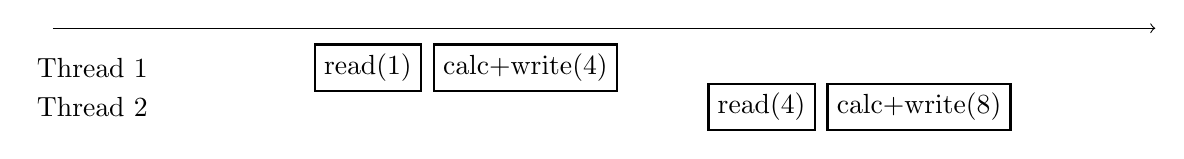
\begin{tikzpicture}
				\path [->] (0,0) edge (14,0);
				
				\node (Thread1) at (0.5,-0.5) {Thread 1};
				\node (Thread2) at (0.5,-1) {Thread 2};
				\begin{scope}[every node/.style={rectangle,thick,draw}]
					\node (read1) at (4,-0.5) {read(1)};
					\node (calcwrite1) at (6,-0.5) {calc+write(4)};
					\node (read2) at (9,-1) {read(4)};
					\node (calcwrite2) at (11,-1) {calc+write(8)};
				\end{scope}
			\end{tikzpicture}
			\hfill \\
			The result with this execution is \textbf{8}.
		\closesection
		\subsection{2. Sequential Execution}
		\startsubsection
			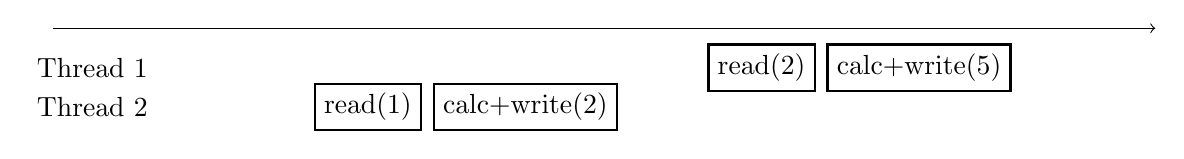
\begin{tikzpicture}
				\path [->] (0,0) edge (14,0);
				
				\node (Thread1) at (0.5,-0.5) {Thread 1};
				\node (Thread2) at (0.5,-1) {Thread 2};
				\begin{scope}[every node/.style={rectangle,thick,draw}]
					\node (read1) at (9,-0.5) {read(2)};
					\node (calcwrite1) at (11,-0.5) {calc+write(5)};
					\node (read2) at (4,-1) {read(1)};
					\node (calcwrite2) at (6,-1) {calc+write(2)};
				\end{scope}
			\end{tikzpicture}
			\hfill \\
			The result with this execution is \textbf{5}.
		\closesection
		\subsection{1. Concurrent Execution}
		\startsubsection
			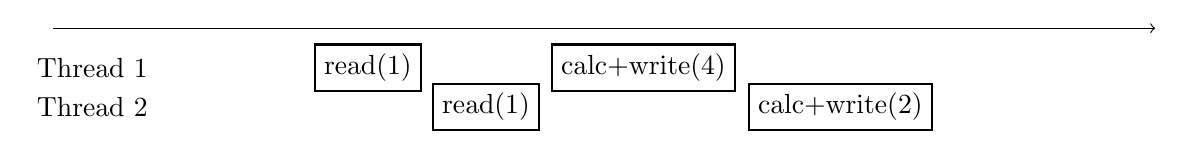
\begin{tikzpicture}
				\path [->] (0,0) edge (14,0);
				
				\node (Thread1) at (0.5,-0.5) {Thread 1};
				\node (Thread2) at (0.5,-1) {Thread 2};
				\begin{scope}[every node/.style={rectangle,thick,draw}]
					\node (read1) at (4,-0.5) {read(1)};
					\node (calcwrite1) at (7.5,-0.5) {calc+write(4)};
					\node (read2) at (5.5,-1) {read(1)};
					\node (calcwrite2) at (10,-1) {calc+write(2)};
				\end{scope}
			\end{tikzpicture}
			\hfill \\
			The result with this execution is \textbf{2}.
		\closesection
		\subsection{2. Concurrent Execution}
		\startsubsection
			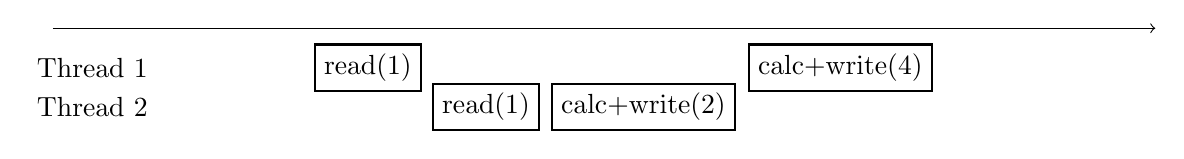
\begin{tikzpicture}
				\path [->] (0,0) edge (14,0);
				
				\node (Thread1) at (0.5,-0.5) {Thread 1};
				\node (Thread2) at (0.5,-1) {Thread 2};
				\begin{scope}[every node/.style={rectangle,thick,draw}]
					\node (read1) at (4,-0.5) {read(1)};
					\node (calcwrite1) at (10,-0.5) {calc+write(4)};
					\node (read2) at (5.5,-1) {read(1)};
					\node (calcwrite2) at (7.5,-1) {calc+write(2)};
				\end{scope}
			\end{tikzpicture}
			\hfill \\
			The result with this execution is \textbf{4}.
		\closesection
		\subsection{3. Concurrent Execution}
		\startsubsection
			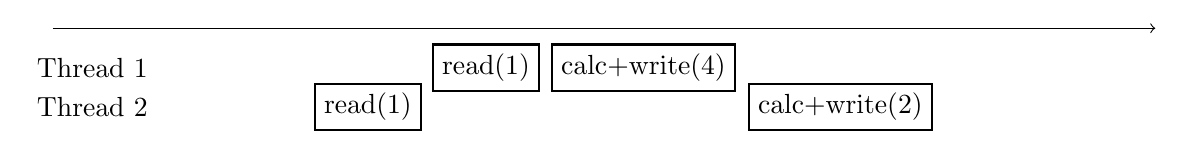
\begin{tikzpicture}
				\path [->] (0,0) edge (14,0);
				
				\node (Thread1) at (0.5,-0.5) {Thread 1};
				\node (Thread2) at (0.5,-1) {Thread 2};
				\begin{scope}[every node/.style={rectangle,thick,draw}]
					\node (read1) at (5.5,-0.5) {read(1)};
					\node (calcwrite1) at (7.5,-0.5) {calc+write(4)};
					\node (read2) at (4,-1) {read(1)};
					\node (calcwrite2) at (10,-1) {calc+write(2)};
				\end{scope}
			\end{tikzpicture}
			\hfill \\
			The result with this execution is \textbf{2}.
		\closesection
		\subsection{4. Concurrent Execution}
		\startsubsection
			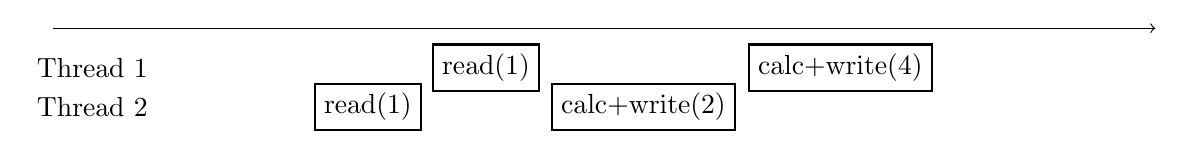
\begin{tikzpicture}
				\path [->] (0,0) edge (14,0);
				
				\node (Thread1) at (0.5,-0.5) {Thread 1};
				\node (Thread2) at (0.5,-1) {Thread 2};
				\begin{scope}[every node/.style={rectangle,thick,draw}]
					\node (read1) at (5.5,-0.5) {read(1)};
					\node (calcwrite1) at (10,-0.5) {calc+write(4)};
					\node (read2) at (4,-1) {read(1)};
					\node (calcwrite2) at (7.5,-1) {calc+write(2)};
				\end{scope}
			\end{tikzpicture}
			\hfill \\
			The result with this execution is \textbf{4}.
		\closesection
	\closesection
	
	\newpage	
	
	\section{Monitor from a Binary Semaphore}
	\startsection
		\begin{minted}{java}
private final Semaphore semaphore = new Semaphore(1)

public void monitor_wrap(Function f) {
	semaphore.acquire()
	try {
		execute f
	} finally { semaphore.release() }
}
		\end{minted}
		\hfill \\
		Every method call in the monitor should call the monitor\textunderscore wrap method with parameter of the method itself, so it is wrapped with a semaphore acquisition and thus mutex is guaranteed.
	\closesection
\end{document}